\documentclass[12pt]{article}         % the type of document and font size (default 10pt)
\usepackage[margin=1.0in]{geometry}   % sets all margins to 1in, can be changed
\usepackage{moreverb}                 % for verbatimtabinput -- LaTeX environment
\usepackage{url}                      % for \url{} command
\usepackage{amssymb}                  % for many mathematical symbols
\usepackage{float}                  % for locking figures in place
\usepackage[pdftex]{lscape}           % for landscaped tables
\usepackage{longtable}    % for tables that break over multiple pages
\usepackage[paper=portrait,pagesize]{typearea}

\usepackage{graphicx} 
\usepackage{subcaption} %  for subfigures environments 
\usepackage{fancyhdr}
\usepackage{xcolor}
\usepackage{lipsum}
%\setlength\headheight{26pt} 
%\rhead{\includegraphics[width=4.25cm]{jpal_logo.png}}
\renewcommand{\headrulewidth}{0pt}


\pagestyle{plain}

\title{Conde Nast Salary Report}  % to specify title
\author{Mike Gibson}          % to specify author(s)
\usepackage{Sweave}
\begin{document} % document begins here

\Sconcordance{concordance:report.tex:report.Rnw:%
1 24 1 1 0 28 1 1 59 2 1 2 4 1 20 1 1 1 4 49 0 1 5 2 1}


% If .nw file contains graphs: To specify that EPS/PDF graph files are to be 
% saved to 'graphics' sub-folder
%     NOTE: 'graphics' sub-folder must exist prior to Sweave step
%\SweaveOpts{prefix.string=graphics/plot}

% If .nw file contains graphs: to modify (shrink/enlarge} size of graphics 
% file inserted
%         NOTE: can be specified/modified before any graph chunk
\setkeys{Gin}{width=.60\textwidth}

\maketitle              % makes the title

\tableofcontents        % inserts TOC (section, sub-section, etc numbers and titles)
%\listoftables           % inserts LOT (numbers and captions)
%\listoffigures          % inserts LOF (numbers and captions)
%                        %     NOTE: graph chunk must be wrapped with \begin{figure}, 
%                        %  \end{figure}, and \caption{}
%%%%%%%%%%%%%%%%%%%%%%%%%%%%%%%%%%%%%%%%%%%%%%%%%%%%%%%%%%%%%%%%%%%%
% Where everything else goes



\bigskip   % leave some empty space (optional)

\section{Salary}

\setkeys{Gin}{width=.8\textwidth}

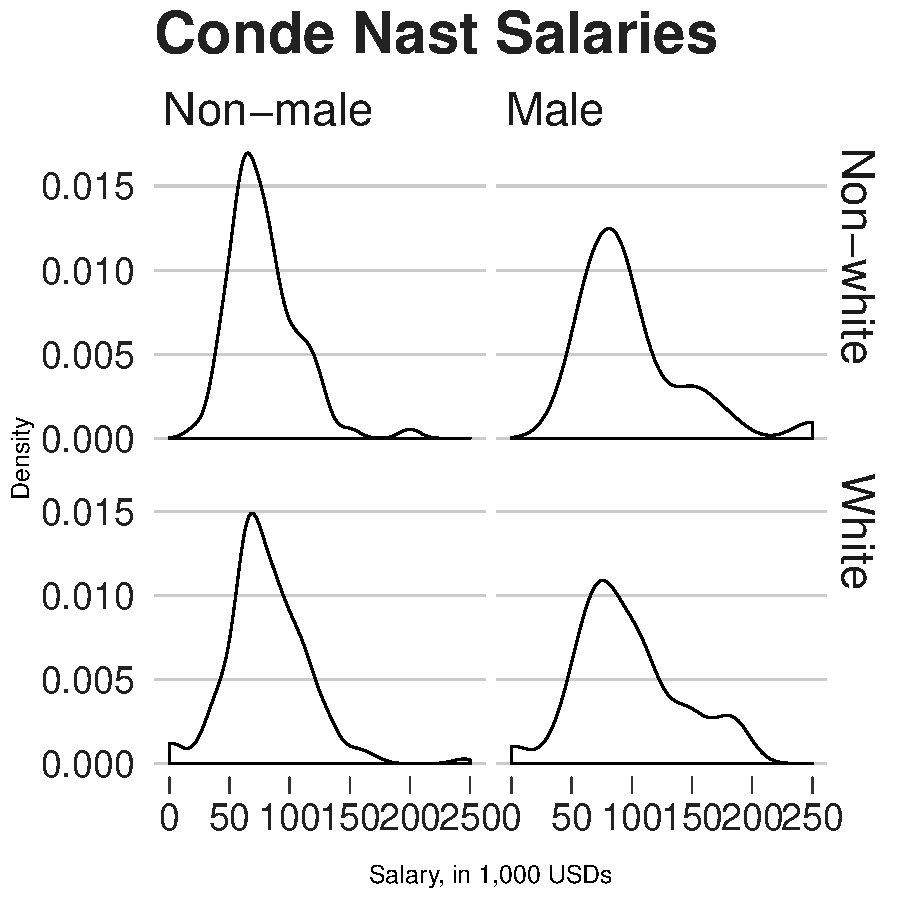
\includegraphics{report-002}



% Table created by stargazer v.5.2.2 by Marek Hlavac, Harvard University. E-mail: hlavac at fas.harvard.edu
% Date and time: Tue, Jun 16, 2020 - 22:21:06
\begin{table}[!htbp] \centering 
  \caption{Predicting Salary} 
  \label{} 
\begin{tabular}{@{\extracolsep{5pt}}lcccc} 
\\[-1.8ex]\hline 
\hline \\[-1.8ex] 
 & \multicolumn{4}{c}{\textit{Dependent variable:}} \\ 
\cline{2-5} 
\\[-1.8ex] & \multicolumn{4}{c}{Salary in 1,000s USD} \\ 
\\[-1.8ex] & (1) & (2) & (3) & (4)\\ 
\hline \\[-1.8ex] 
 White & 0.886 & 0.917 & 0.973 & $-$0.426 \\ 
  & (4.031) & (4.033) & (4.008) & (3.835) \\ 
  & & & & \\ 
 Male & 17.623$^{***}$ & 17.819$^{***}$ & 14.398$^{***}$ & 14.936$^{***}$ \\ 
  & (4.427) & (4.435) & (4.535) & (4.366) \\ 
  & & & & \\ 
 Straight & 7.084 & 6.668 & 5.357 & 6.721 \\ 
  & (4.550) & (4.577) & (4.556) & (4.363) \\ 
  & & & & \\ 
 Cisgendered & 19.838$^{*}$ & 19.723$^{*}$ & 20.545$^{**}$ & 15.871 \\ 
  & (10.329) & (10.334) & (10.235) & (9.804) \\ 
  & & & & \\ 
 Full Time &  & 5.714 & 3.197 & $-$0.751 \\ 
  &  & (6.703) & (6.693) & (6.423) \\ 
  & & & & \\ 
 Years of Experience &  &  & $-$0.576 & $-$0.193 \\ 
  &  &  & (0.361) & (0.351) \\ 
  & & & & \\ 
 Years in Current Role &  &  & 2.684$^{**}$ & 2.648$^{***}$ \\ 
  &  &  & (1.061) & (1.013) \\ 
  & & & & \\ 
 Direct reports &  &  &  & 3.870$^{***}$ \\ 
  &  &  &  & (1.054) \\ 
  & & & & \\ 
 Indirect Reports &  &  &  & 1.984$^{**}$ \\ 
  &  &  &  & (0.916) \\ 
  & & & & \\ 
 Constant & 55.029$^{***}$ & 50.179$^{***}$ & 54.613$^{***}$ & 49.605$^{***}$ \\ 
  & (9.889) & (11.413) & (11.968) & (11.467) \\ 
  & & & & \\ 
\hline \\[-1.8ex] 
Observations & 331 & 331 & 331 & 331 \\ 
R$^{2}$ & 0.070 & 0.073 & 0.099 & 0.184 \\ 
\hline 
\hline \\[-1.8ex] 
\textit{Note:}  & \multicolumn{4}{r}{$^{*}$p$<$0.1; $^{**}$p$<$0.05; $^{***}$p$<$0.01} \\ 
\end{tabular} 
\end{table} 

\end{document}
